%Testen und Dokumentieren wird wie ein Stiefkind behandelt. Warum ist es sinnvoll, diese Themen im Informatikunterricht st�rker hervorzustreichen? Mit Zope 3 ist dieser Ansatz sehr sch�n zu realisieren, da er vom Framework und der Art der Implementierung unterst�tzt wird.
Testen und Dokumentieren von Software gewinnt erst bei gro�en Softwareprojekten an Relevanz. Dementsprechend wird das Testen von Software im Unterricht vernachl�ssigt, da nur in seltenen F�llen gro�e Projekte realisiert werden, bei denen das Testen unerl�sslich wird. 
Bei kleinen Projekten ist es auch schwer, den doch enormen Aufwand vor den Studenten zu rechtfertigen. Die Fehler scheinen bei normaler Benutzung der Software viel schneller gefunden zu werden.

Selbst in der Industrie scheint es, als ob das Testen von Software nicht durchg�ngig als wichtiges Element im Softwareentwicklungsprozess gesehen wird. Eine Studie aus dem Jahr 2003 \cite{misc:testingsurvey} besagt, dass 52\% der befragten Softwareentwickler ihren Code testen, 34\% manchmal und 14\% �berhaupt nicht. Testen wird als l�stiges und langweiliges Anh�ngsel gesehen. Hier ist ein deutlicher Nachholbedarf ersichtlich. Nach Erfahrung des Autors ist das nur theoretisch in die Lehre vorgedrungen, die praktische Anwendung kommt jedoch zu kurz.

\begin{quote}
{\itshape "'Developers reuse code but do not test it to the
extent we expected [...] simple to use tools are lacking when it comes to test creation and test analysis [...] knowledge on the importance of testing in general and \emph{unit} testing in particular seem low"'}\cite{misc:testingsurvey}
\end{quote}

Entwickler testen so gut wie keine Reuse-Implementierung. Gerade bei der Zunahme an Reuse und der Komponentenorientierung von Software verlagert sich die Relevanz von der Entwicklung zum Testen. Die Komponenten selbst m�ssen mit Tests ausgeliefert werden, und die Benutzung dieser erfordert weitere Integrationstests. Weiters werden Tools zur Erstellung und Validierung von Tests als unbefriedigend empfunden. Die Wichtigkeit der Thematik wird generell untersch�tzt.

Im Folgenden werden die unterschiedlichen Testm�glichkeiten mit \Zope\ besprochen. Eine tats�chliche Umsetzung davon wird in der Beispielimplementierung, Kapitel \ref{kapitel:Beispielimplementierung} pr�sentiert. Weiters wird auf das \emph{doctesting}, einer Testmethode mit gleichzeitiger Dokumentation eingegangen.
  
\paragraph*{Unit Tests}

Ein \emph{Unit test} ist ein White-Box Test, wobei nur eine spezielle Komponente f�r sich allein getestet wird. Der Test wird von der Umwelt (wie andere Komponenten) nicht beeinflusst. Er testet die kleinste �berhaupt testbare Einheit (Unit) einer Software. Ziel ist die Funktionalit�t jeder einzelnen Komponente zu garantieren. Nach dem \TDD\/ \cite{952753} werden \emph{Unit tests} vor der Programmierung einer Komponente entwickelt, die Funktionalit�t der Komponente wird dann f�r den Test entwickelt (siehe Abbildung \ref{fig:TDD}). Dieses Vorgehen zwingt den Entwickler, sich im Vorfeld intensiver mit der gew�nschten Funktionalit�t einer Komponente auseinanderzusetzen. Dabei wird im Vorfeld das \API\ durch die Testf�lle definiert und danach implementiert.

\begin{figure}[h]
	\centering
	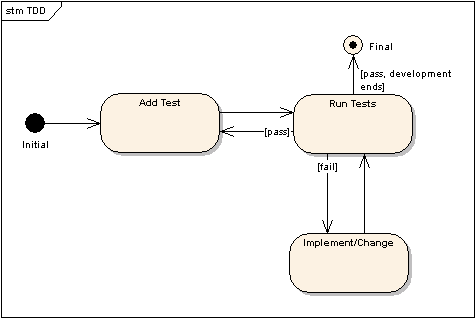
\includegraphics[scale=0.7]{graphics/TDD.png}
	\caption{Test Driven Development (TDD)}
	\label{fig:TDD}
\end{figure}

Python wird mit dem \verb|unittest| Modul\footnote{PyUnit: http://pyunit.sourceforge.net/} ausgeliefert und ist die Pythonvariante von \emph{JUnit}\footnote{JUnit: http://junit.org/}, bekannt aus der Java-Welt. Das Modul kann somit unter \Zope\ verwendet werden.

Nachfolgend ist ein einfacher Testcase mit dem \verb|unittest| Modul unter Python dargestellt:

\begin{lstlisting}[style=interpreter]
>>> import unittest
>>> class MyTestCase(unittest.TestCase):
...		def test_TwoMinusThree(self):
...			self.assertEqual(2 - 3, -1)
...			self.failIfEqual(2 - 3, 1)
...		
>>> unittest.main()
\end{lstlisting}

\paragraph*{Integration Tests und Functional Tests}

\emph{Integration tests} testen die Interaktion zwischen Komponenten, f�r die schon erfolgreich laufende \emph{Unit tests} geschrieben wurden. Dabei wird zum ersten Mal das Zusammenspiel der Komponenten in einem gemeinsamen Kontext getestet. Die n�chste Steigerung ist der Functional Test, bei dem das System als Black-Box betrachtet wird. Die Tests laufen aus der Sicht eines Benutzers.

\begin{quote}
{\itshape "'[...] in the Zope world, functional tests are really integration tests. Functional tests would treat Zope like a black box. "'Functional tests"' in Zope, however, do not simulate a browser client program and connect through the \HTTP\ port. They only simulate the necessary objects, such as the browser request. That means, they are more like integration tests."'}\cite{zope:weitershausen}
\end{quote}

Unter Zope gibt es keine Trennung der beiden Testbegriffe. Es wird unkorrekterweise einheitlich von \emph{Functional tests} gesprochen.

\paragraph*{Doctests}  

\emph{Doctesting} ist eine eigene Art Pythons, Dokumentation mit Tests zu verschmelzen. �blicherweise sind Tests selbst schon eine gute Dokumentation, wenn man die Funktionalit�t einer Komponente verstehen will. Meist sind sie aber nicht gerade komfortabel zu lesen. 

\begin{quote}
{\itshape "'Doctest is a system for writing tests within Python documentation strings.
The emphasis is on documentation. Tests are provided as example code, set
off with Python prompts. Doctest tests lend themselves toward a literate form
of test code."'}\cite{misc:pycon2004doctest}
\end{quote}

Ein \emph{Doctest} wird entweder in den \emph{Docstring}\footnote{Docstring: http://en.wikipedia.org/wiki/Docstring} im Quelltext geschrieben, oder als eigenes Textfile abgelegt. Letzteres empfiehlt sich bei umfangreicher Testl�nge. Aus den \emph{Docstrings} k�nnen seperate Dokumentationen, z.B. als \HTML\ oder \PDF\/ extrahiert werden. \emph{Doctests} werden im Stil einer Interpreter Session geschrieben. Erkl�rende Worte dazu sind im \emph{reStructuredText} Format\footnote{reStructuredText: http://docutils.sourceforge.net/rst.html} zu w�hlen. Listing \ref{python:doctest} zeigt ein kurzes Beispiel zur Veranschaulichung.

\begin{lstlisting}[style=example, caption={Doctest from the Zope 3 SessionCredentials Plugin}, label=python:doctest]
...
class SessionCredentials(object):
    """Credentials class for use with sessions.

    A session credential is created with a login and a password:

      >>> cred = SessionCredentials('scott', 'tiger')

    Logins are read using getLogin:
    
      >>> cred.getLogin()
      'scott'

    and passwords with getPassword:

      >>> cred.getPassword()
      'tiger'

    """
    def __init__(self, login, password):
        self.login = login
        self.password = password
        
    def getLogin(self): return self.login
    def getPassword(self): return self.password
...
\end{lstlisting}


\emph{Doctests} k�nnen  \emph{Unit tests} und \emph{Integration tests} in einem besser les- und schreibbaren Format abbilden.  Der Entwickler kann anhand einer "'Erz�hlung"' seinen Quelltext dokumentieren und zugleich testen. Die Vorteile liegen auf der Hand. Die Handhabung schl�gt zwei Fliegen mit einer Klappe und ist leichter zu erlernen als z.B. das \emph{Unit test} \API\/. Diese Art von Dokumentationstest erscheint dem Autor ein gutes Werkzeug, um die Thematik Testen und Dokumentieren im Unterricht darzulegen.

%Zope3 Teststrategie Zope philisophy
%Zope besteht aus xx tests..

%automatisierung